\chapter{Zahlen und Wirklichkeit}
\label{chap:II_zahlen}
\label{chap:II_grundlagen}
\setcounter{section}{2}
\setcounter{subsection}{0}
\setcounter{secnumdepth}{3}

% =====================================================
% 2.1 Natürliche Zahlen und Zählen
% =====================================================

\subsection{Natürliche Zahlen und Zählen}
\label{sec:2.1_natuerliche_zahlen}

Die Geschichte der \emph{Zahlen}\index{Zahlen} beginnt mit dem Bedürfnis des Menschen, 
seine Umwelt zu ordnen. 
Lange bevor es \emph{Schrift}\index{Schrift} oder 
\emph{Rechenverfahren}\index{Rechenverfahren} gab, 
nutzte man das \emph{Zählen}\index{Zählen}, um Tiere, Werkzeuge oder Tage festzuhalten. 
Das Zählen war eine grundlegende \emph{Kulturtechnik}\index{Kulturtechnik}, 
ohne die \emph{Handel}\index{Handel}, 
\emph{Planung}\index{Planung} und 
\emph{Wissenschaft}\index{Wissenschaft} 
nicht denkbar gewesen wären.

\subsubsection*{Früheste Ansätze}
\phantomsection
Archäologische Funde\index{Archäologie} deuten darauf hin, dass bereits vor 
rund 20.000 bis 35.000 Jahren \emph{Zählhilfen}\index{Zählhilfen} benutzt wurden. 
Besonders bekannt ist der \emph{Ishango-Knochen}\index{Ishango-Knochen}, 
entdeckt 1960 von Jean de Heinzelin de Braucourt\index{Heinzelin de Braucourt, Jean de} 
in Zentralafrika. 
Noch älter ist das \emph{Lebombo-Knochenstück}\index{Lebombo-Knochen} 
aus Südafrika. Beide Artefakte belegen, dass Menschen schon in der 
\emph{Altsteinzeit}\index{Altsteinzeit} 
mit Einkerbungen Mengen darstellten (vgl.~Abb.~\ref{fig:knochen}). 

\begin{figure}[ht]
	\centering
	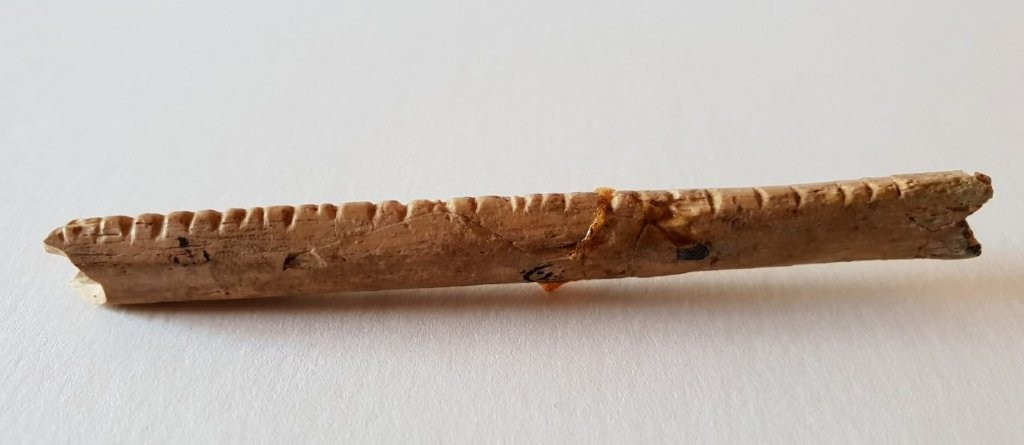
\includegraphics[width=0.45\textwidth]{bilder/lebombo-bone.png}
	\hfill
	\includegraphics[width=0.45\textwidth]{bilder/ishango_bone.jpg}
	\caption{Links: Lebombo-Knochenstück (ca.\ 35.000 Jahre alt, Südafrika). 
		Rechts: Ishango-Knochen (ca.\ 20.000 Jahre alt, Zentralafrika). 
		Beide zeigen regelmäßige Einkerbungen, die als frühe Zählhilfen gedeutet werden. 
		Der Ishango-Knochen wird heute im \emph{Königlichen Belgischen Institut für Naturwissenschaften} in Brüssel aufbewahrt.}
	\label{fig:knochen}
\end{figure}

\HistoryBox{Der Ishango-Knochen}{box:ishango}{%
	Der \emph{Ishango-Knochen} wurde 1960 von 
	Jean de Heinzelin de Braucourt in Zentralafrika entdeckt und ist etwa 20.000 Jahre alt. 
	
	Auf dem Knochen finden sich drei Spalten von Einkerbungen, 
	die nicht zufällig verteilt sind, sondern in Gruppen geordnet erscheinen. 
	Wahrscheinlich diente er als eine Art \emph{Zählstab}\index{Zählstab} – 
	möglicherweise zur Beobachtung des \emph{Mondzyklus}\index{Mondzyklus} 
	oder zur Zählung von Vorräten.
	
	Besonders auffällig: Einige Gruppierungen entsprechen \emph{Primzahlen}\index{Primzahlen} 
	(11, 13, 17, 19). Ob dies Zufall oder Absicht war, bleibt offen. 
	Der Knochen zeigt jedoch, dass Menschen schon in der Altsteinzeit 
	Zahlen nutzten, um Muster in ihrer Welt zu erkennen und festzuhalten.
}

Auch andernorts nutzten Menschen Einkerbungen, Knoten oder Steine als einfache Zählhilfen. 
Kerbhölzer dienten über Jahrtausende zur Aufzeichnung von Vorräten, Abgaben oder Schulden – 
bis in die Neuzeit hinein, etwa im Alpenraum. 
Überall griff man unabhängig zur gleichen Idee: 
Einkerbungen als elementare Zählhilfe.

\subsubsection*{Vom Zählen zum Zahlbegriff}
\phantomsection
Neben archäologischen Funden zeigt auch die \emph{Sprachforschung}\index{Sprachforschung}, 
dass Menschen ihre Umwelt zunächst nur grob in kleine und große Mengen unterteilten – 
anfangs: \emph{eins}, \emph{zwei}, \emph{viele}. 

Manche traditionellen Kulturen kennen bis heute nur sehr wenige \emph{Zahlwörter}\index{Zahlen}, 
oft lediglich die Unterscheidung \glqq eins\grqq, \glqq zwei\grqq{} und \glqq viele\grqq, 
etwa in \emph{Papua-Neuguinea}\index{Papua-Neuguinea} oder \emph{Australien}\index{Australien}. 

Das zeigt: \emph{Zahlen}\index{Zahlen} sind keine Selbstverständlichkeit, 
sondern eine kulturelle \emph{Erfindung}, entstanden aus praktischen Bedürfnissen 
wie \emph{Handel}\index{Handel}, \emph{Vorratshaltung}\index{Vorratshaltung} 
oder \emph{Kalenderrechnung}\index{Kalenderrechnung}. 

Überall – in Afrika, Asien, Europa oder Ozeanien – entwickelten Menschen Zählhilfen 
und \emph{Zahlbegriffe}\index{Zahlbegriff}. 
Das Bedürfnis, die Welt in Zahlen zu fassen, spiegelt eine tiefe Struktur der 
\emph{Wirklichkeit}\index{Wirklichkeit} wider.



% =====================================================
% 2.2 Irrationale Zahlen – die Krise der Griechen
% =====================================================

\subsection{Irrationale Zahlen – die Krise der Griechen}
\label{sec:2.2_irrat}

\subsubsection*{Ausgangspunkt: Pythagoras und die Pythagoreer}
\phantomsection
Die frühen griechischen Mathematiker\index{Griechen}, vor allem die Schule der 
\emph{Pythagoreer}\index{Pythagoreer}, waren überzeugt, dass sich die Welt vollständig 
durch \emph{ganze Zahlen}\index{ganze Zahlen} und \emph{Brüche}\index{Brüche} beschreiben lässt. 
Ihr Leitsatz lautete: „Alles ist Zahl.“ 
Der \emph{Satz des Pythagoras}\index{Satz des Pythagoras} war dafür das zentrale Symbol.

\subsubsection*{Erste Erkenntnisse: Inkommensurabilität}
\phantomsection
Beim Quadrat mit Seitenlänge $1$ wollten die Pythagoreer die Länge der Diagonale berechnen. 
Nach dem Satz des Pythagoras gilt:
\[
c^2 = 1^2 + 1^2 = 2 \quad \Rightarrow \quad c = \sqrt{2}.
\]

Die Zahl $\sqrt{2}$ ließ sich jedoch durch keinen Bruch zweier ganzer Zahlen darstellen. 
Damit war klar: Es gibt \emph{inkommensurable Längen}\index{inkommensurabel}, 
die kein gemeinsames Maß besitzen. 
Die Seitenlänge $1$ und die Diagonale $\sqrt{2}$ sind inkommensurabel.
Diese Erkenntnis stellte die Grundüberzeugung der Pythagoreer in Frage, 
dass die Welt ausschließlich durch ganze Zahlen und Brüche erklärbar sei.

\subsubsection*{Die Krise der Griechen}
\phantomsection
Die Entdeckung der Irrationalität stürzte die Pythagoreer in eine intellektuelle Krise.  
Der Überlieferung nach soll \emph{Hippasos von Metapont}\index{Hippasos von Metapont} 
diese Tatsache erkannt haben – 
die Legende berichtet sogar, dass er von seinen Brüdern ertränkt wurde, 
weil er dieses „Geheimnis“ preisgab. 
Ob die Geschichte wahr ist oder nicht: 
Sicher ist, dass die Entdeckung der Irrationalität 
die griechische Mathematik tief erschütterte. 

\subsubsection*{Der Beweis}
\phantomsection
Einen strengen Beweis für die Irrationalität formulierte \emph{Euklid}\index{Euklid} 
im 10.~Buch seiner \emph{Elemente}\index{Elemente (Euklid)}. 
Er basiert auf einem klassischen Widerspruchsargument:

\MatheBox{Widerspruchsbeweis für $\sqrt{2}$}{box:beweis_wurzel2}{%
	Angenommen, $\sqrt{2}$ sei rational, also $\sqrt{2}=\tfrac{p}{q}$ mit 
	ganzen Zahlen $p,q$, die teilerfremd sind. 
	Dann gilt $2q^2=p^2$. 
	Daraus folgt: $p^2$ ist gerade, also ist auch $p$ gerade. 
	Schreiben wir $p=2r$, dann gilt $2q^2=(2r)^2=4r^2$, also $q^2=2r^2$. 
	Damit ist auch $q$ gerade. 
	
	Somit sind $p$ und $q$ beide gerade, also nicht teilerfremd. 
	Dies widerspricht der Annahme. 
	Damit ist $\sqrt{2}$ irrational.
}

Anschaulich bedeutet dies: 
Es gibt kein gemeinsames Maß, 
mit dem man gleichzeitig die Seitenlänge $1$ und die Diagonale $\sqrt{2}$ 
genau abmessen könnte. 
Jeder Bruch führt irgendwann in einen Widerspruch. 
$\sqrt{2}$ gehört also nicht zur Welt der Brüche, 
sondern eröffnet die neue Zahlenwelt der \emph{irrationalen Zahlen}\index{irrationale Zahlen}.
Die ausführliche Herleitung des Beweises findet sich in 
Anhang~\ref{anhangA_wurzel2}.

\subsubsection*{Näherungen und Berechnung}
\phantomsection
Trotz der Irrationalität blieb $\sqrt{2}$ unverzichtbar. 
Darum entwickelten verschiedene Kulturen Verfahren, den Wert möglichst genau zu bestimmen.

\paragraph{Indische Näherung (Śulba-Sūtras).}
In den altindischen \emph{Śulba\-/Sūtras}\index{Śulba-Sūtras}\index{Indien!Mathematik}
findet sich eine berühmte Näherungsregel für $\sqrt{2}$:
\[
\sqrt{2}\approx 1+\frac{1}{3}+\frac{1}{3\cdot 4}\;-\;\frac{1}{3\cdot 4\cdot 34}
\;=\;1.414\,215\ldots
\]
Schon sechs Nachkommastellen stimmen mit dem exakten Wert überein.

\paragraph{Griechische Verfahren: Iteration und Kettenbruch.}
Arithmetisch nutzten die Griechen das Verfahren 
$x_{n+1}=\tfrac{1}{2}(x_n+\tfrac{2}{x_n})$, 
das rasch zu $\sqrt{2}$ konvergiert – 
heute bekannt als \emph{Newton-Verfahren}.  
Geometrisch wurde die sogenannte \emph{Anthyphairesis} verwendet, 
eine frühe Form des Kettenbruchs:
\[
\sqrt{2}=[1;\overline{2}]=1+\cfrac{1}{2+\cfrac{1}{2+\cdots}}
\]
Die Konvergenten ($3/2,\ 7/5,\ 17/12,\dots$) liefern immer bessere Bruchnäherungen; 
das periodische Muster $\overline{2}$ macht die Irrationalität sichtbar.

\HinweisBox{Mathematik als Entdeckung}{box:mathematik_entdeckung}{%
	Die Entdeckung der irrationalen Zahlen war ein Wendepunkt: 
	Zahlen sind keine bloßen Erfindungen, sondern beschreiben Strukturen, 
	die in der Natur tatsächlich vorkommen. 
	Das Quadrat mit Seitenlänge $1$ „erzwingt“ die Existenz von $\sqrt{2}$.
}

% =====================================================
% 2.3 Null und negative Zahlen
% =====================================================

\subsection{Null und negative Zahlen}
\label{sec:2.3_null_negative}

\subsubsection*{Einleitung}
\phantomsection
Die Vorstellung von \emph{Nichts}\index{Nichts} als Zahl und die Idee von \emph{negativen Zahlen}\index{negative Zahlen} 
sind für uns heute selbstverständlich. 
Historisch jedoch war ihre Entwicklung lang und von Widerständen begleitet. 
Für viele Kulturen war es kaum vorstellbar, 
dass es eine Zahl für „nichts“ geben sollte – oder gar für „weniger als nichts“. 

\subsubsection*{Die Null – Zahl aus dem Nichts}
\phantomsection
Schon die Babylonier nutzten ein Platzhaltersymbol, wenn eine Stelle leer blieb. 
Eine wirkliche \emph{Null als Zahl} entwickelte sich jedoch erst in Indien.  
Dort formulierte \textbf{Brahmagupta}\index{Brahmagupta} im Jahr 628 n.\,Chr. erstmals Rechenregeln mit $0$ 
(in seinem \emph{Brahmasphutasiddhanta}).  
Über die arabische Welt gelangte das Konzept nach Europa und wurde 
durch \textbf{Leonardo Fibonacci}\index{Fibonacci, Leonardo} in seinem \emph{Liber Abaci} (1202) verbreitet.

Viele Philosophen und Theologen taten sich mit der Null schwer. 
Wie konnte „Nichts“ eine Zahl sein? 
In Europa galt sie lange als verdächtig oder sogar gefährlich, 
da sie mit der Idee des Abgrunds oder des Nichtseins verbunden war.  
Heute ist die Null Grundlage des Stellenwertsystems und 
unverzichtbar für die moderne Mathematik.

\subsubsection*{Negative Zahlen – Schulden und Temperaturen}
\phantomsection
Negative Zahlen tauchten bereits in China um 200 v.\,Chr. auf, 
in den \emph{Neun Büchern über die Mathematik}\index{China!Neun Bücher über die Mathematik}.  
Man unterschied positive und negative Werte mit verschiedenfarbigen Rechenstäbchen: 
rot für Gewinne, schwarz für Verluste.  
Auch in Indien wurden negative Zahlen verwendet, etwa zur Darstellung von Schulden oder Defiziten. 

\begin{figure}[ht]
	\centering
	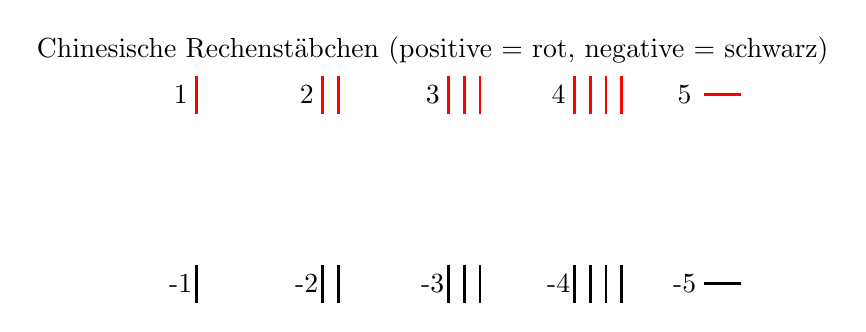
\begin{tikzpicture}[scale=0.8, line width=1pt]
		\node at (4,3.2) {Chinesische Rechenstäbchen (positive = rot, negative = schwarz)};
		% Positive Zahlen (rot)
		\foreach \n/\count in {1/1, 2/2, 3/3, 4/4} {
			\node at (2*\n-2,2.5) {\n};
			\foreach \i in {1,...,\count} {
				\draw[red] (2*\n-2+0.25*\i,2.2) -- (2*\n-2+0.25*\i,2.8);
			}
		}
		\node at (8,2.5) {5};
		\draw[red] (8.3,2.5) -- (8.9,2.5);
		% Negative Zahlen (schwarz)
		\foreach \n/\count in {1/1, 2/2, 3/3, 4/4} {
			\node at (2*\n-2,-0.5) {-\n};
			\foreach \i in {1,...,\count} {
				\draw[black] (2*\n-2+0.25*\i,-0.8) -- (2*\n-2+0.25*\i,-0.2);
			}
		}
		\node at (8,-0.5) {-5};
		\draw[black] (8.3,-0.5) -- (8.9,-0.5);
	\end{tikzpicture}
	\caption{Chinesische Rechenstäbchen: positive Zahlen (rot), negative Zahlen (schwarz).}
	\label{fig:rod_numerals_colored}
\end{figure}

\MatheBox{Rechenregeln für negative Zahlen}{box:regeln_negative}{%
	Heute sind die Regeln vertraut:
	\[
	(+a)+(-b)=a-b, \quad (-a)+(-b)=-(a+b),
	\]
	\[
	(-a)\cdot(-b)=+ab, \quad (-a)\cdot b=-(ab).
	\]
	Doch diese einfachen Regeln wurden in Europa erst sehr spät akzeptiert. 
	\textbf{René Descartes}\index{Descartes, René} bezeichnete negative Zahlen noch als 
	„falsche Zahlen“.
}

Viele Mathematiker fragten sich: 
Wie kann man „weniger als nichts“ besitzen? 
Ein negatives Ergebnis schien absurd. 
Erst durch praktische Anwendungen wie Buchhaltung (Schulden) oder 
Temperaturmessungen unter Null wurde ihre Nützlichkeit offensichtlich.
Mit der Null und den negativen Zahlen erweiterte sich das Zahlensystem entscheidend: 
Mathematik begann, nicht nur das Zählen von Dingen zu beschreiben, 
sondern auch Abwesenheit und Gegensätze. 
So entstand die moderne Zahlengerade, 
auf der sich alle ganzen Zahlen von $-\infty$ bis $+\infty$ anordnen lassen.

% =====================================================
% 2.4 Komplexe Zahlen – eine unerwartete Erweiterung
% =====================================================

\subsection{Komplexe Zahlen – eine unerwartete Erweiterung}
\label{sec:2.4_komplexe}

\subsubsection*{Einleitung}
\phantomsection
Während Brüche, irrationale Zahlen, die Null und die negativen Zahlen jeweils aus praktischen 
Problemen hervorgegangen sind, entstand die nächste Erweiterung des Zahlbegriffs fast beiläufig: 
die sogenannten \emph{komplexen Zahlen}.  
Sie tauchten auf, als man versuchte, Gleichungen zu lösen, 
die mit den bekannten Zahlenarten nicht lösbar waren.

\subsubsection*{Erste Ansätze in der Renaissance}
\phantomsection
Im 16.~Jahrhundert beschäftigten sich italienische Mathematiker wie 
\textbf{Scipione del Ferro}\index{del Ferro, Scipione}, 
\textbf{Niccolò Tartaglia}\index{Tartaglia, Niccolò} und 
\textbf{Gerolamo Cardano}\index{Cardano, Gerolamo} mit kubischen Gleichungen.  
Bei manchen Lösungswegen traten Zwischenschritte mit $\sqrt{-1}$ auf – 
obwohl das Endergebnis wieder eine reelle Zahl war.  
Cardano nannte diese Ausdrücke „sophistische Wurzeln“ – 
er schrieb sie zwar auf, verstand sie aber nicht.  
Man hielt sie für eine Art Rechenkuriosität: notwendig im Lösungsweg, 
aber ohne eigenständige Bedeutung.

\subsubsection*{Bombelli und die Wende}
\phantomsection
Der italienische Mathematiker \textbf{Rafael (Raffaele) Bombelli}\index{Bombelli, Rafael} erkannte um 1572, 
dass man mit diesen „imaginären Zahlen“ konsistent rechnen kann, 
wenn man sie wie gewöhnliche Zahlen behandelt und $i^2=-1$ setzt.  
Damit legte er den Grundstein für die Theorie der komplexen Zahlen.

Noch lange galten komplexe Zahlen als „fiktiv“ oder „imaginär“.  
Erst im 18.~und 19.~Jahrhundert, bei \textbf{Leonhard Euler}\index{Euler, Leonhard}, 
\textbf{Carl Friedrich Gauss}\index{Gauss, Carl Friedrich} und 
\textbf{Jean-Robert Argand}\index{Argand, Jean-Robert}, 
setzte sich die Erkenntnis durch:  
Komplexe Zahlen sind nicht nur Hilfsmittel, sondern eine 
notwendige und vollwertige Erweiterung des Zahlbegriffs.  

\subsubsection*{Bedeutung}
\phantomsection
Heute bilden die komplexen Zahlen ein Fundament der modernen Mathematik.  
Sie garantieren mit dem \emph{Fundamentalsatz der Algebra}\index{Fundamentalsatz der Algebra}, 
dass jedes Polynom eine Lösung besitzt, 
und sind in Physik und Technik unverzichtbar – etwa für Schwingungen, Wellen, 
Quantenmechanik und Elektrotechnik.

Die ausführliche historische Herleitung und die formale Einführung von $i^2=-1$ 
finden sich im Anhang~\ref{anhangA_i}.

% =====================================================
% 2.5 Fazit
% =====================================================

\subsection{Fazit: Zahlen als entdeckte Struktur}

Vom Zählen der Herden bis zur Einführung der komplexen Zahlen zeigt sich ein roter Faden: 
Neue Zahlenarten entstehen nicht willkürlich, sondern immer dann, wenn die bisherigen 
Zahlen nicht mehr ausreichen.  

\begin{itemize}
	\item Die \emph{natürlichen Zahlen}\index{natürliche Zahlen} entstanden aus dem praktischen Bedürfnis zu zählen.  
	\item \emph{Irrationale Zahlen}\index{irrationale Zahlen} wurden entdeckt, als die Geometrie den Bereich der Brüche sprengte.  
	\item Die \emph{Null}\index{Null} und die \emph{negativen Zahlen}\index{negative Zahlen} öffneten den Blick für Abwesenheit und Gegensätze.  
	\item Die \emph{komplexen Zahlen}\index{komplexe Zahlen} machten scheinbar unlösbare Gleichungen lösbar und führten zur Vollständigkeit der Mathematik.  
\end{itemize}

\HinweisBox{Zahlen als universelle Struktur}{box:mathematik_entdeckung_fazit}{%
	Zahlen sind keine freie Erfindung des Menschen.  
	Sie wurden Schritt für Schritt \emph{entdeckt}, weil die Welt selbst 
	eine innere Struktur hat, die wir in Zahlen fassen können.  
	Durch logisches Weiterdenken und konsequentes Rechnen erschlossen sich immer neue Zahlbereiche – 
	von den Kerben auf Knochen bis hin zur komplexen Ebene.  
}
